\clearpage
\chapter{Metodología}

\section{Desarrollo ágil de software}
  \paragraph{El desarrollo ágil propone una alternativa al desarrollo de software tradicional. Los enfoques del desarrollo ágil son principalmente usados en el desarrollo de software para ayudar a las compañias a responder fácilmente al cambio.}\cite{22}

\subsection{Scrum}
  \paragraph{Scrum es un marco de gestión para el desarrollo incremental de un producto que proporciona una estructura de roles, reuniones, reglas y artefactos.}
  \paragraph{Scrum utiliza iteraciones de longitud fija denominados Sprints, que son típicamente de dos semanas o 30 días de duración. Los equipos de Scrum intentan generar un incremento de producto potencialmente entregable (debidamente probado) en cada iteración.}\cite{23}
  
  \begin{center}
    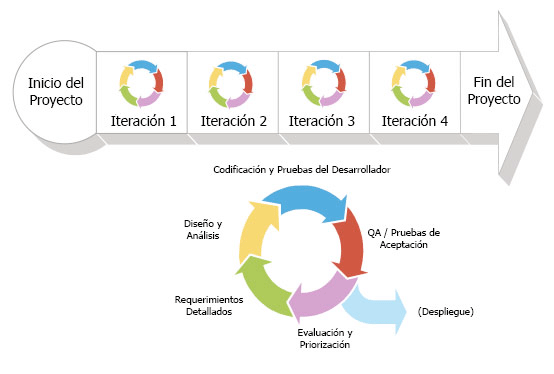
\includegraphics[width=14cm, height=9cm]{images/iterations}
  \end{center}

 \subsection{Programación Extrema (XP)}
  \paragraph{Es un enfoque disciplinado para entregar software de alta calidad rápida y continuamente. Promueve una alta participación del cliente, retroalimentación rápida, pruebas continuas, planeación continua y entrega de software funcional en intervalos muy frecuentes que van de 1 a 3 semanas.}\cite{24}
  
\section{Técnicas de desarrollo ágil}

\subsection{Desarrollo guiado por pruebas (Test Driven Development)}

  \paragraph{El desarrollo guiado por pruebas es una técnica avanzada qua hace uso de pruebas unitarias para guiar el diseño del software y forzar el desacoplamiento de dependencias.}
  \paragraph{El resultado de usar esta práctica es una comprensiva suite de pruebas que pueden ser ejecutadas en cualquier momento para proporcionar información de que el software está aún funcionando.}\cite{25}

\subsection{Refactor}
  \paragraph{Es una técnica disciplinada para la reestructuración de un cuerpo de código existente, alterando su estructura interna sin cambiar su comportamiento exterior.}
  \paragraph{Cada transformación es pequeña, pero una secuencia de transformaciones pueden producir una importante reestructuración.}\cite{26}

\subsection{Integración continua}
  \paragraph{Es una práctica de desarrollo que requiere a los desarrolladores la integración de código en un repositorio compartido varias veces al día.}
  \paragraph{Cada registro de entrada es entonces verificado por un proceso de construcción automatizado permitiendo a los equipos detectar problemas a tiempo.}
  \paragraph{La integración continua trae muchos beneficios, entre ellos la detección de errores rápidamente y reducir los problemas de integración lo que permite entrega de software más rápidamente.}\cite{27}

\section{Justificación}

  \paragraph{Para el desarrollo del sistema pondrémos en práctica las técnicas mencionadas anteriormente que son características del marco de trabajo Scrum y de la metodología Extreme Programming.}

  \paragraph{El proceso de desarrollo del proyecto se llevará a cabo de la siguiente manera:}

  \begin{itemize}
    \item Planteamiento de las historias de usuario.
    \item Definción del plazo de tiempo para cada sprint y el conjunto de funcionalidades relacionadas a cada historia de usuario que serán desarrolladas dentro del mismo.  
    \item Implementación de pruebas unitarias en conjunto con el desarrollo de cada módulo de la aplicación. 
    \item Implementación de pruebas de integración para verificar la comunicación entre dos o más modulos.
    \item Despliegue de la aplicación en un ambiente productivo una vez que todas las pruebas hayan pasado.
    \item Implementación de pruebas funcionales para verificar que el flujo descrito en las historias de usuario se lleva a cabo correctamente.
  \end{itemize}

\section{Modelo por prototipos}
  \paragraph{Es un modelo para el desarrollo de sistemas en el cual un prototipo es construido, probado y finalmente reconstruido las veces que sea necesario hasta que un prototipo aceptable es finalmente alcanzado del cual el sistema completo o producto puede ser totalmente desarrollado.}

  \paragraph{Este modelo funciona bien en escenarios donde no se conocen por completo los requerimientos.}

\subsection{¿Qué es un prototipo de software?}
  \paragraph{Es un modelo de software con una funcionalidad limitada que permite al usuario evaluar los propósitos del desarrollador y probarlos antes de su implementación.}
  \paragraph{También ayuda a entender los requerimientos específicos del usuario y que no pudieron haber sido considerados por el desarrollador durante el diseño del sistema.}

\subsection{Implementación del modelo de prototipos}
\begin{itemize}
  \item Los nuevos requerimientos del sistema se definen con el mayor detalle posible.
  \item Un diseño preeliminar es creado para el nuevo sistema. 
  \item Un primer prototipo del nuevo sistema es construido para el diseño preeliminar que representa una aproximación a las características del producto final.
  \item El usuario evalua el primer prototipo, notando sus fortalezas y debilidades, qué necesita agregarse y que debería removerse. El usuario recoge las observaciones de los usuarios. 
  \item El primer prototipo es modificado, basado en los comentarios hechos por el usuario, y un segundo prototipo del nuevo sistema es construido.
  \item El segundo prototipo es evaluado del mismo modo que el primero.
  \item Los pasos anteriores son iterados tantas veces como sea necesario, hasta que los usuarios consideren que el prototipo representa al producto final deseado.
  \item El sistema final es construido, basado en el prototipo final.
  \item El sistema final es evaluado y probado a fondo. Existe una rutina de mantenimiento continuo para prevenir errores a gran escala.
\end{itemize}
